\chapter{Implementasi dan Pengujian}
\label{chapter:implementasiPengujian}
Bab ini membahas tentang implementasi dan pengujian perangkat lunak berdasarkan rancangan yang telah dibuat. Terdapat dua jenis pengujian yang dilakukan yaitu pengujian fungsional dan pengujian eksperimental. Kemudian pada bab ini juga dibahas tentang lingkungan yang digunakan untuk pengujian perangkat lunak ini.

\section{Lingkungan untuk Implementasi dan Pengujian}
Terdapat dua lingkungan yang digunakan untuk implementasi dan pengujian. Lingkungan pertama digunakan untuk implementasi serta pengujian fungsi-fungsi dari aplikasi. Sedangkan lingkungan kedua digunakan untuk melakukan pengujian eksperimental. Berikut ini merupakan spesifikasi lingkungan perangkat keras dan juga perangkat lunak yang digunakan:
\begin{enumerate}
	\item Lingkungan pertama, berikut ini merupakan spesifikasi lingkungan pertama:
		\begin{table}[h!]
		\centering
		\begin{tabular}{|| m{16em} | m{20em} ||} 
 		\hline
		{\bf Parameter} & {\bf Nilai} \\ [0.5ex] 
 		\hline\hline
		{\it Processor} & 1.8 GHz Intel Core i5 \\ 
		\hline
		{\it Graphics Processing Unit} (GPU) & Intel HD Graphics 6000 1536 MB  \\ 
		\hline
		{\it Random Access Memory} (RAM) & 8 GB 1600 MHz DDR3 \\ 
		\hline
		{\it Storage} & 121 GB SSD \\ [1ex] 
 		\hline
		\end{tabular}
		\caption{Lingkungan perangkat keras lingkungan pertama.}
		\label{table:1}
		\end{table}
		
		\begin{table}[h!]
		\centering
		\begin{tabular}{|| m{16em} | m{20em} ||} 
 		\hline
		{\bf Parameter} & {\bf Nilai} \\ [0.5ex] 
 		\hline\hline
		Sistem Operasi & macOS Sierra \\ 
		\hline
		Bahasa Pemrograman & JavaScript, CSS, dan HTML  \\ 
		\hline
		{\it Text Editor} (RAM) & Visual Studio Code \\ 
 		\hline
		Perangkat lunak pendukung & MAMP version: 4.2.1 dan Google Chrome Version 64.0.3282.186 (Official Build) (64-bit) \\ [1ex] 
 		\hline
		\end{tabular}
		\caption{Lingkungan perangkat lunak lingkungan pertama.}
		\label{table:1}
		\end{table}
		
	\item Lingkungan kedua, berikut ini merupakan spesifikasi lingkungan kedua:
		\begin{table}[h!]
		\centering
		\begin{tabular}{|| m{16em} | m{20em} ||} 
 		\hline
		{\bf Parameter} & {\bf Nilai} \\ [0.5ex] 
 		\hline\hline
		{\it Processor} & 1.8 GHz Intel Core i5 \\ 
		\hline
		{\it Graphics Processing Unit} (GPU) & Intel HD Graphics 6000 1536 MB  \\ 
		\hline
		{\it Random Access Memory} (RAM) & 8 GB 1600 MHz DDR3 \\ 
		\hline
		{\it Storage} & 121 GB SSD \\ [1ex] 
 		\hline
		\end{tabular}
		\caption{Lingkungan perangkat keras lingkungan pertama.}
		\label{table:1}
		\end{table}
		
		\begin{table}[h!]
		\centering
		\begin{tabular}{|| m{16em} | m{20em} ||} 
 		\hline
		{\bf Parameter} & {\bf Nilai} \\ [0.5ex] 
 		\hline\hline
		Sistem Operasi & macOS Sierra \\ 
		\hline
		Bahasa Pemrograman & JavaScript, CSS, dan HTML  \\ 
		\hline
		{\it Text Editor} (RAM) & Visual Studio Code \\ 
 		\hline
		Perangkat lunak pendukung & MAMP version: 4.2.1 dan Google Chrome Version 64.0.3282.186 (Official Build) (64-bit) \\ [1ex] 
 		\hline
		\end{tabular}
		\caption{Lingkungan perangkat lunak lingkungan pertama.}
		\label{table:1}
		\end{table}
\end{enumerate}

\section{Implementasi}
\label{sec:implementasi}
Pada bagian ini akan dijelaskan hasil implementasi yang dilakukan pada aplikasi sesuai dengan rancangan pada bab sebelumnya.

\subsection{Kode Program}
\label{sec:kodeprogram}
Pengimplementasian Aplikasi Pratinjau 3 Dimensi Berbasis Web dilakukan dalam bahasa pemrograman JavaScript. Kode program untuk masing-masing fitur akan dijabarkan berikut ini:
\begin{itemize}
	\item {\bf Fitur mengganti warna dinding dan lantai ruangan kelas}.
	Potongan kode program pada implementasian fitur berdasarkan rancangan yang telah dibuat sebelumnya dapat dilihat pada gambar ~\ref{fig:implementasidinding} dan ~\ref{fig:implementasilantai}.
	\begin{figure}[ht]
		\centering
		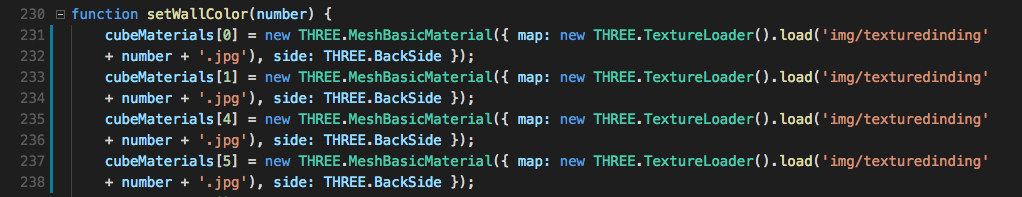
\includegraphics[scale=0.42]{fiturwarnadinding}
		\caption{Kode program fitur mengganti warna dinding ruangan kelas.}
		\label{fig:implementasidinding}
	\end{figure}
	
	\begin{figure}[!hb]
		\centering
		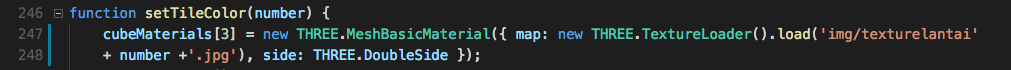
\includegraphics[scale=0.42]{fiturwarnalantai}
		\caption{Kode program fitur mengganti warna lantai ruangan kelas.}
		\label{fig:implementasilantai}
	\end{figure}
	\item {\bf Fitur unggah berkas JavaScript Object Notation (JSON) pada menambah dan mengganti isi informasi ruangan kelas}.
	Potongan kode program pada implementasi fitur berdasarkan rancangan yang telah dibuat sebelumnya dapat dilihat pada gambar ~\ref{fig:implementasiunggahjson}. Namun kode lengkap keseluruhan hanya dapat dilihat pada lampiran.
	\begin{figure}[ht]
		\centering
		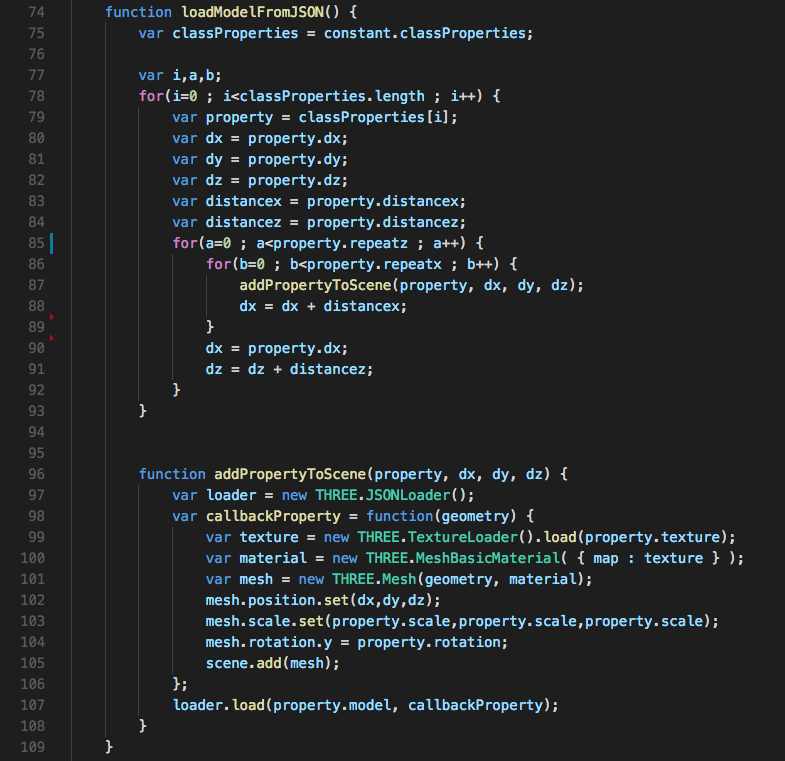
\includegraphics[scale=0.42]{fiturupload}
		\caption{Kode program fitur unggah berkas JSON.}
		\label{fig:implementasiunggahjson}
		\vspace{8mm}
		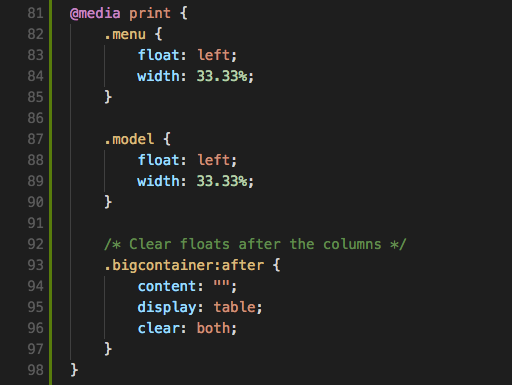
\includegraphics[scale=0.42]{fiturresponsif}
		\caption{Kode program fitur halaman web yang responsif.}
		\label{fig:implementasiweb}
	\end{figure}
	\item {\bf Fitur Halaman Web yang Responsif}.
	Potongan kode program pada implementasi fitur berdasarkan rancangan yang telah dibuat sebelumnya dapat dilihat pada gambar ~\ref{fig:implementasiweb}. Potongan kode ini merupakan pengaturan tampilan pada berkas dengan ekstensi CSS.
\end{itemize}

\subsection{Tampilan}
\label{sec:tampilan}
Pengimplementasian tampilan pada Aplikasi Pratinjau 3 Dimensi Berbasis Web sesuai dengan yang telah dirancang sebelumnya dapat dilihat pada gambar ~\ref{fig:tampilan}.
\begin{figure}[ht]
	\centering
	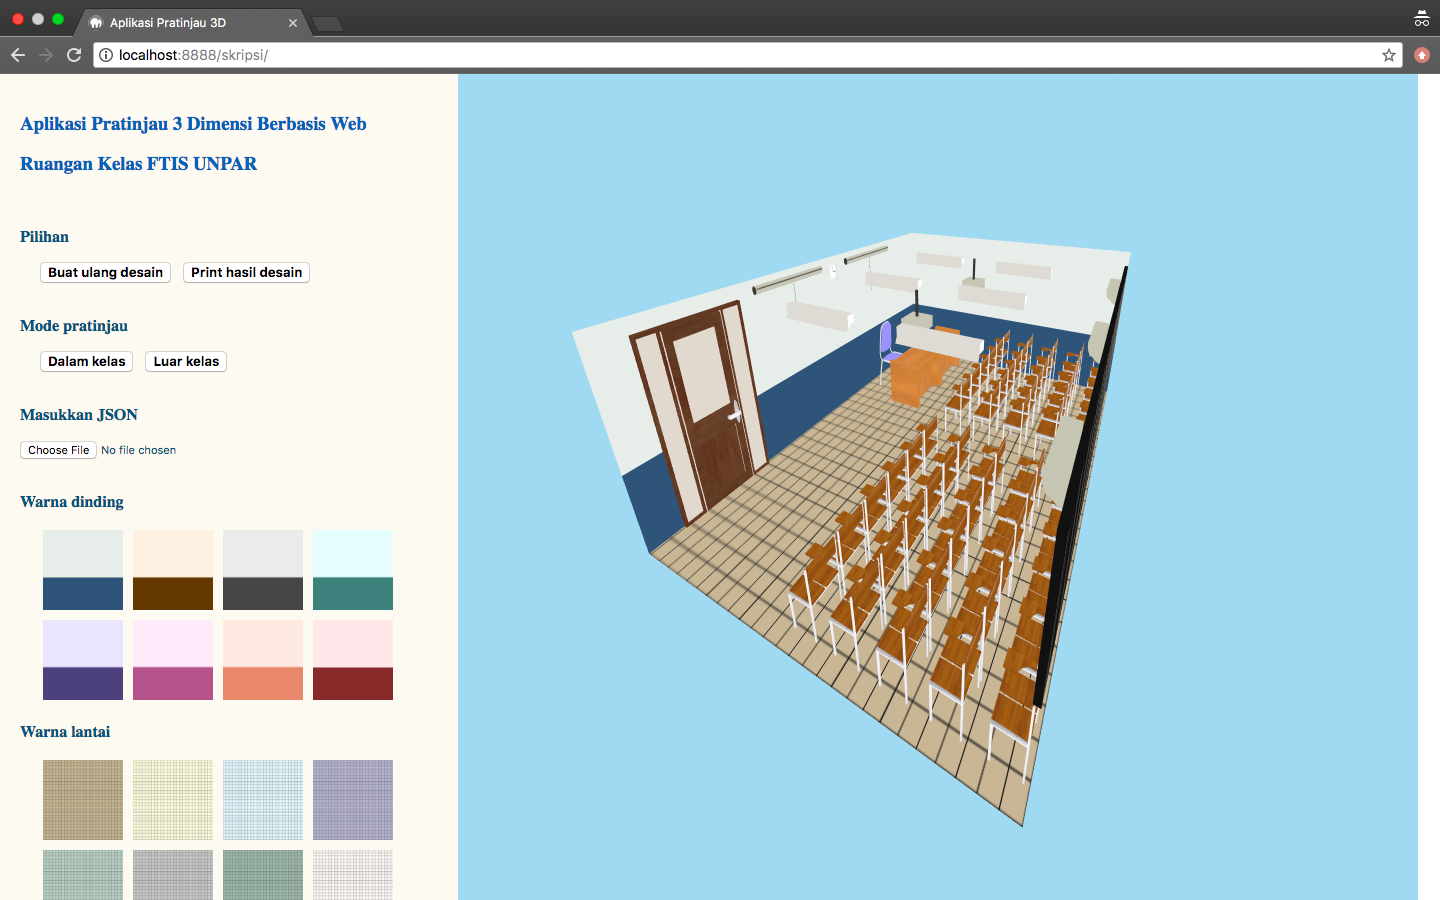
\includegraphics[scale=0.3]{tampilan}
	\caption{Tampilan akhir dari web.}
	\label{fig:tampilan}
\end{figure}

\section{Pengujian Fungsional}
\label{sec:pengujianFungsional}
Pengujian fungsional dilakukan untuk memastikan bahwa Aplikasi Pratinjau 3 Dimensi Berbasis Web telah berjalan dengan baik.

\subsection{Mengganti Tekstur Warna Dinding dan Lantai Ruangan Kelas}
\label{sec:gantitekstur}
Hasil yang diharapkan dari pengujian fitur ini adalah tekstur warna pada dinding dan lantai model ruangan kelas Fakultas Teknologi Informasi dan Sains dapat berubah sesuai dengan pilihan pengguna seperti yang sudah dirancang pada ~\ref{sec:fiturgantiwarna}. Pengujian ini dilakukan dengan memilih salah satu tekstur yang tersedia untuk masing-masing dinding dan lantai pada pilihan di bagian kiri halaman web. Contoh hasil pengujian fitur ini dapat dilihat pada gambar ~\ref{fig:gantitekstur1} dan ~\ref{fig:gantitekstur2}.
\begin{figure}[ht]
	\centering
	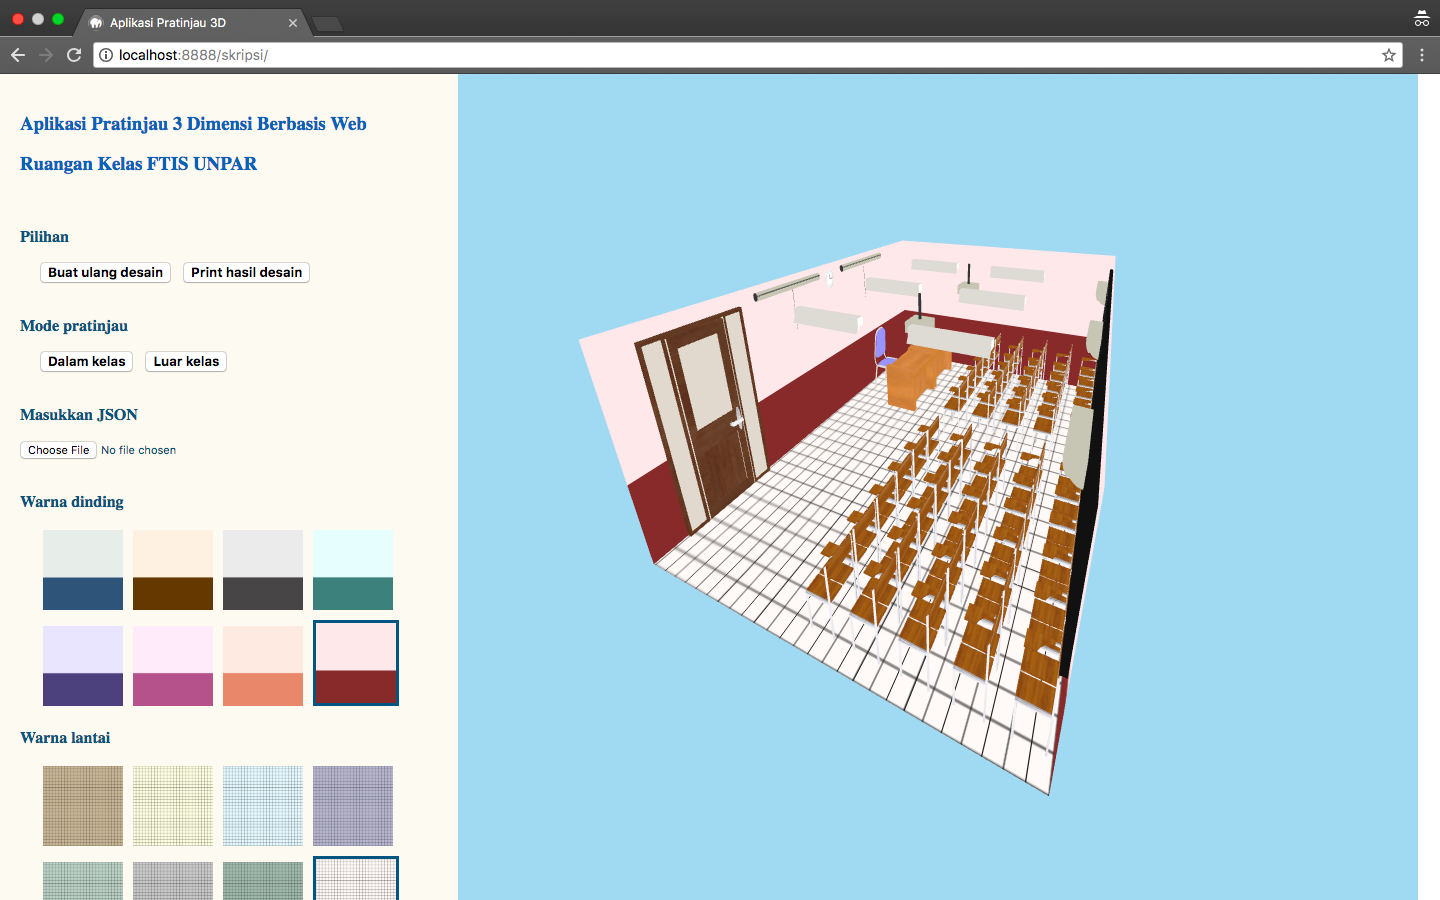
\includegraphics[scale=0.3]{gantitekstur1}
	\caption{Pengujian mengganti tekstur warna dinding dan lantai ruangan kelas.}
	\label{fig:gantitekstur1}
	\vspace{8mm}
	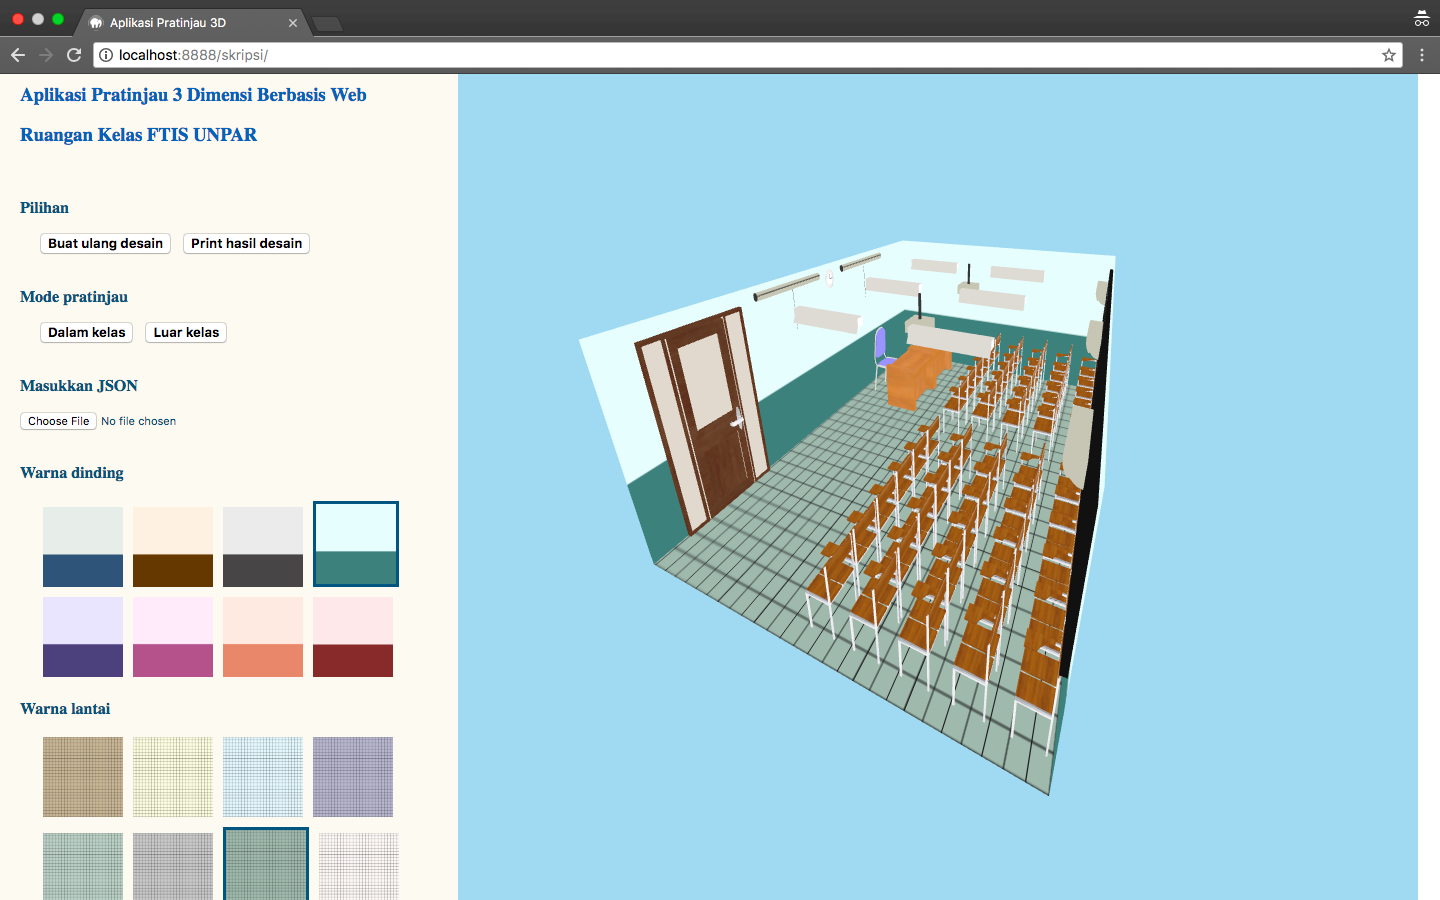
\includegraphics[scale=0.3]{gantitekstur2}
	\caption{Pengujian mengganti tekstur warna dinding dan lantai ruangan kelas.}
	\label{fig:gantitekstur2}
\end{figure}

\subsection{Mengunggah Berkas JSON untuk Mengubah Informasi Isi Ruangan Kelas}
\label{sec:unggahjson}
Hasil yang diharapkan dari pengujian fitur ini adalah hasil unggahan berkas JSON dapat teraplikasikan ke pemodelan ruangan kelas pada aplikasi. Pengujian ini dilakukan dengan menghapus seluruh properti kelas dan hanya menyisakan satu buah kursi mahasiswa di tengah-tengah ruangan kelas. Contoh hasil pengujian fitur ini dapat dilihat pada gambar ~\ref{satukursi}.
 \begin{figure}
	\centering
	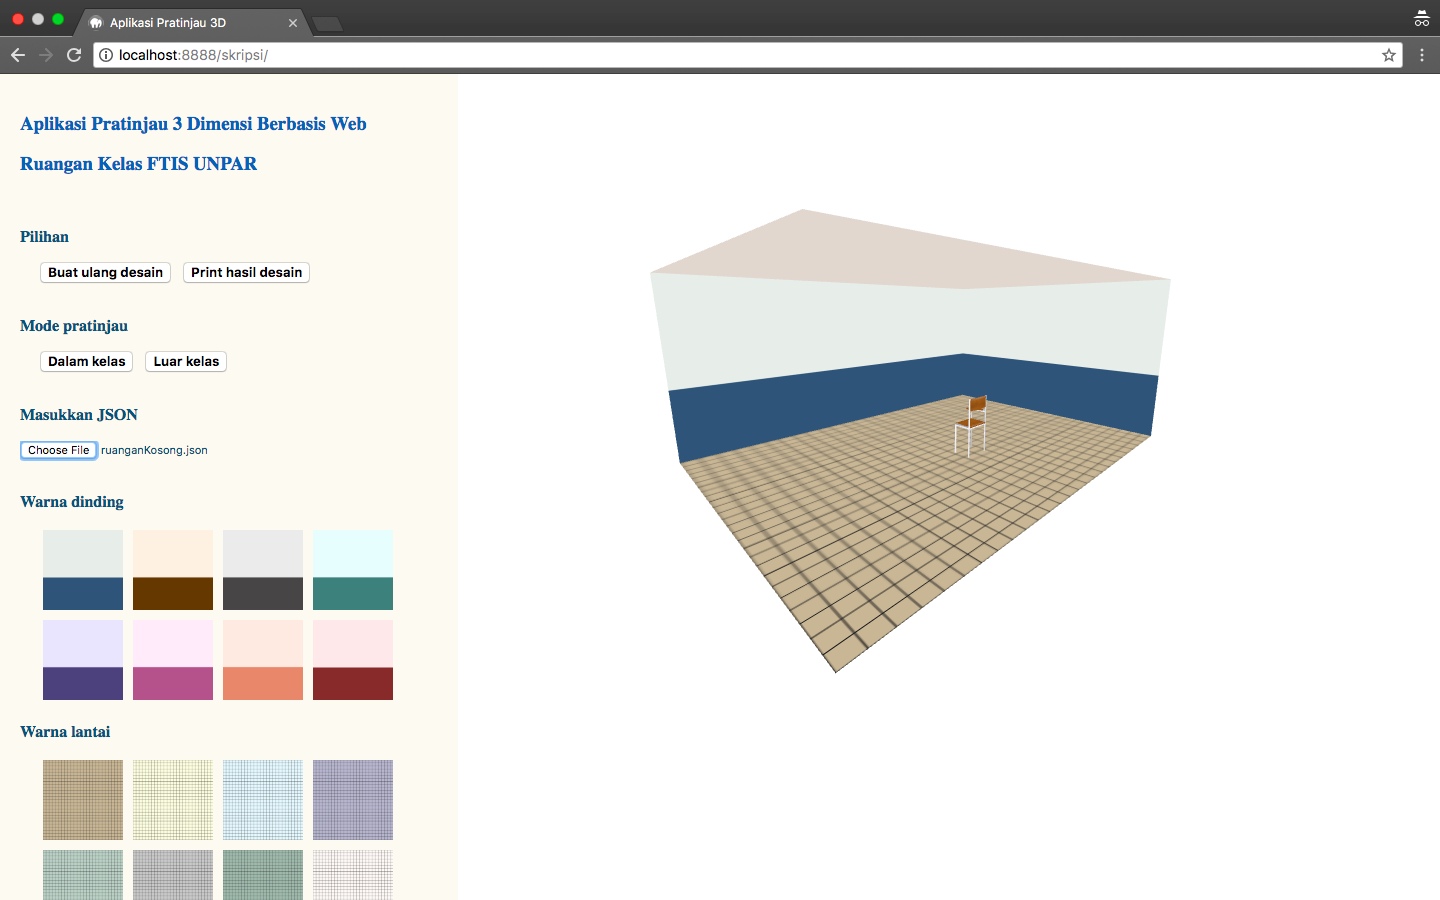
\includegraphics[scale=0.3]{satukursi}
	\caption{Pengujian menyisakan satu kursi di tengah ruangan kelas.}
	\label{fig:satukursi}
\end{figure}
















